\newcommand{\posterBeamProfile}[1]{

\setlength{\frameWidth}{#1}
\setlength{\unitlength}{0.02\frameWidth}
\psset{unit=\unitlength}


\rput[t](12,32){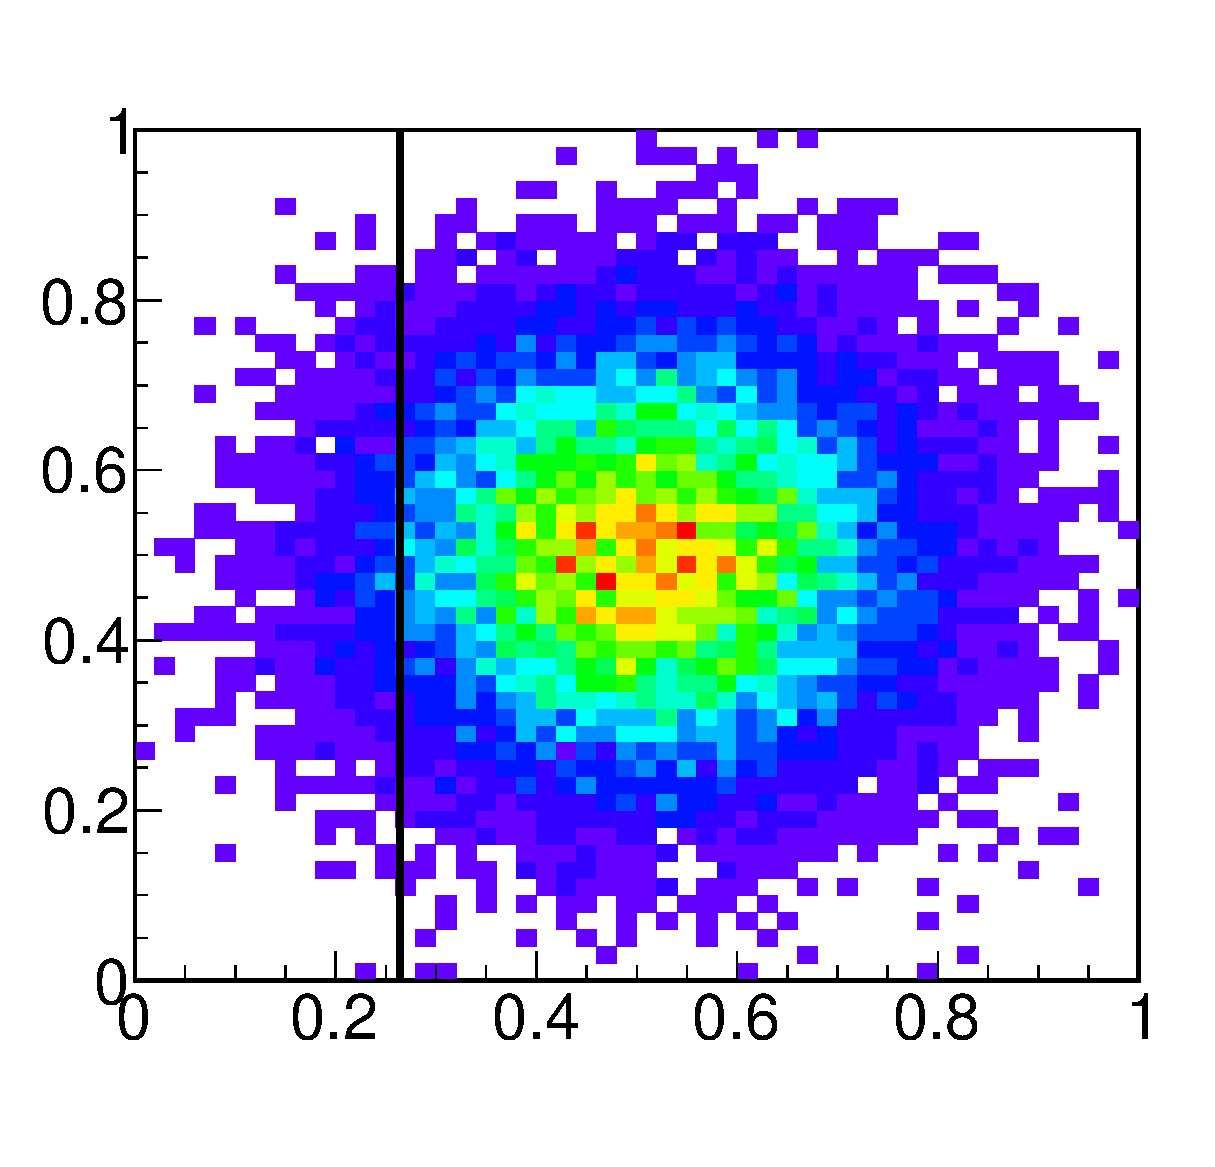
\includegraphics[height=18\unitlength]{graphics/profile_0170}}
\rput[t](38,15){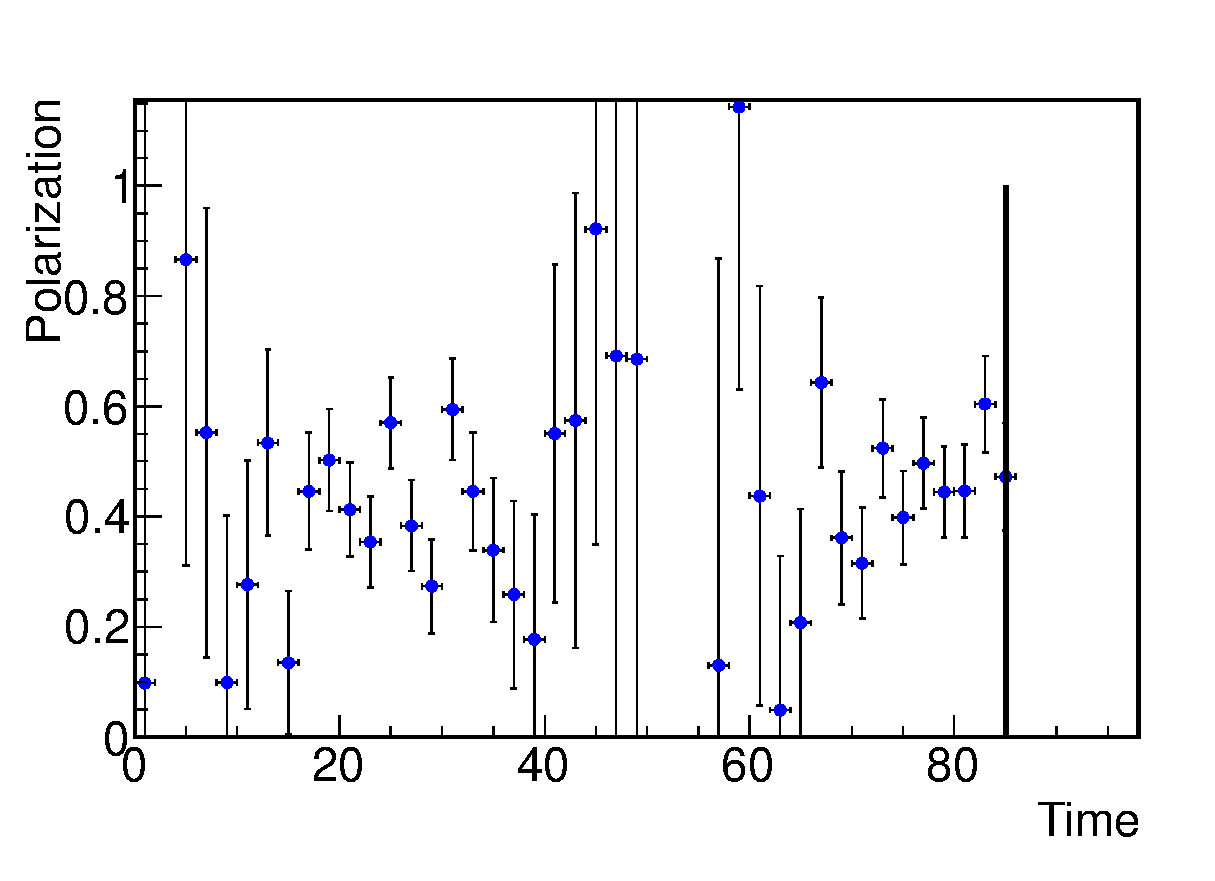
\includegraphics[height=18\unitlength]{graphics/polar_0170}}
\rput[t](38,32){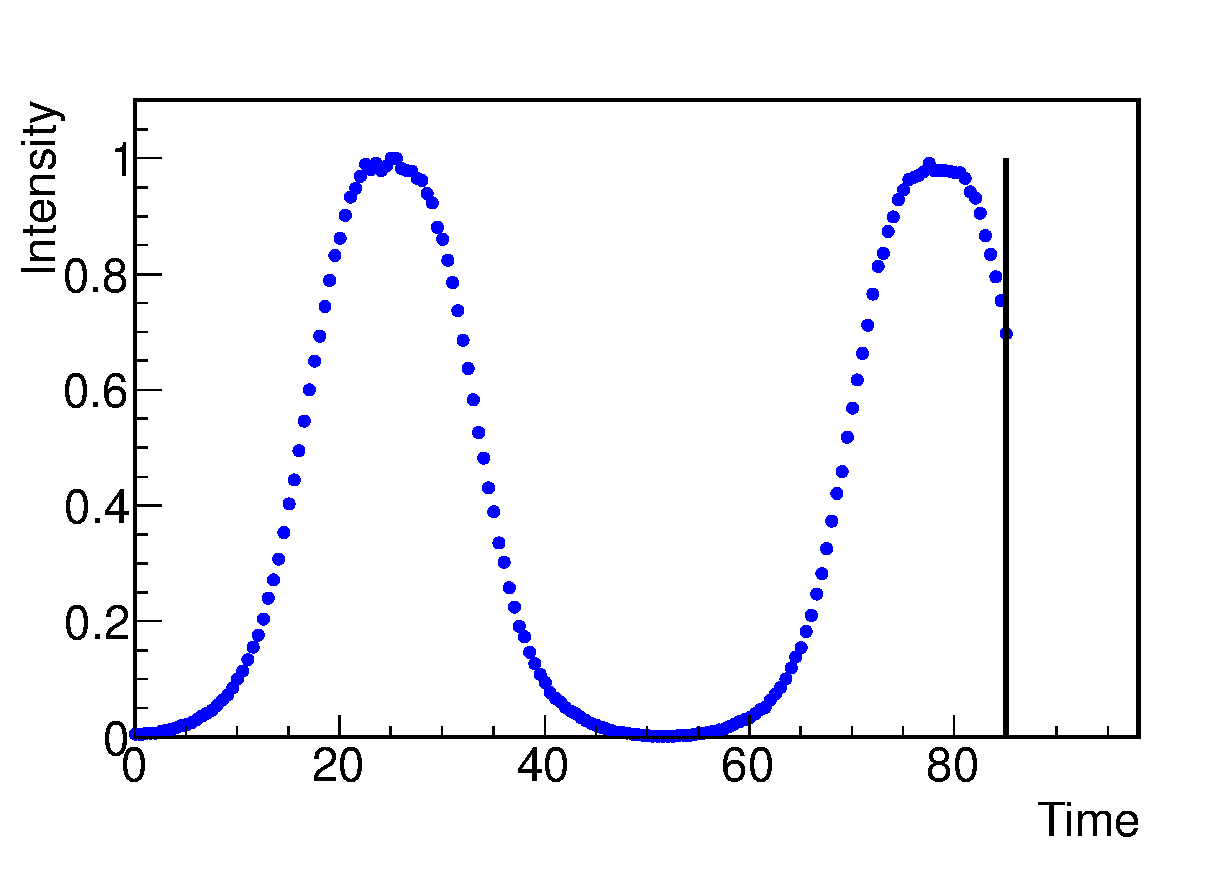
\includegraphics[height=18\unitlength]{graphics/intens_0170}}


\rput[lb](1,1) {%
\begin{minipage}{23\unitlength}
\raggedright
\begin{list}{\labelitemi}{\setlength{\itemsep}{-5mm}\setlength{\leftmargin}{2\unitlength}
                          \setlength{\topsep}{0mm}}

   \item Polarization and intensity profile can be described with
   gaussian distributions:
   %
   \begin{equation*}
   P = P_\text{max} e^{- \frac{\vec{x}^2}{\sigma^2_P}}, \hspace{2\unitlength}
   I = I_\text{max} e^{- \frac{\vec{x}^2}{\sigma^2_I}}
   \end{equation*}

   \item Profile parameter \psframebox{$R = \frac{\sigma^2_I}{\sigma^2_P}$}

\end{list}
\end{minipage}
}


%\rput{0}{\psgrid[gridlabels=0.7,subgriddiv=0, griddots=3](1,-1)(0,0)(\myPsPictureWidthLocal,\myPsPictureHeightLocal)}

}

\setlength{\unitlength}{10mm}
\psset{unit=\unitlength}
